\begin{figure}
	\centering
	\begin{subfigure}[b]{0.2\textwidth}
		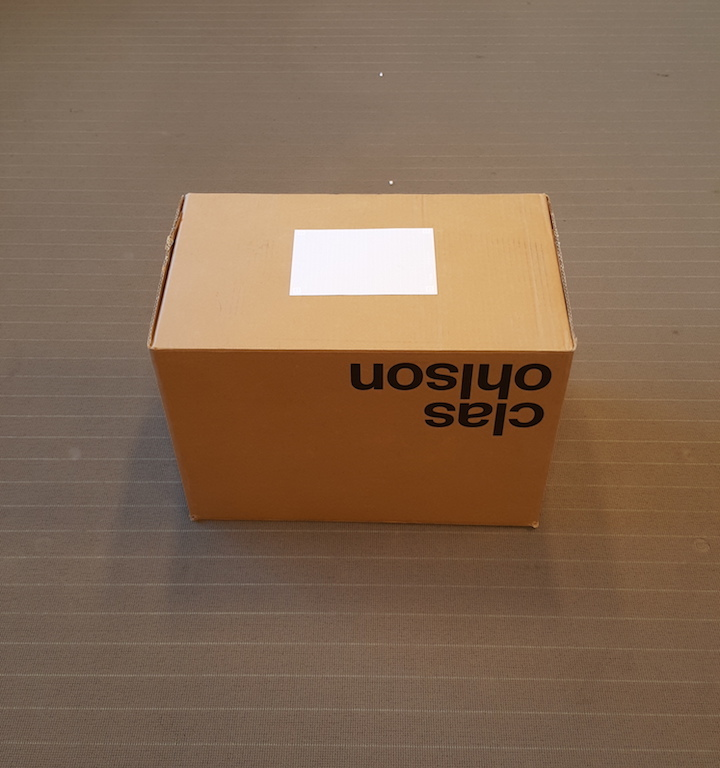
\includegraphics[width=\textwidth]{figures/angle_1.jpg}
		\label{fig:angle_1}
	\end{subfigure}
	~
	\begin{subfigure}[b]{0.2\textwidth}
		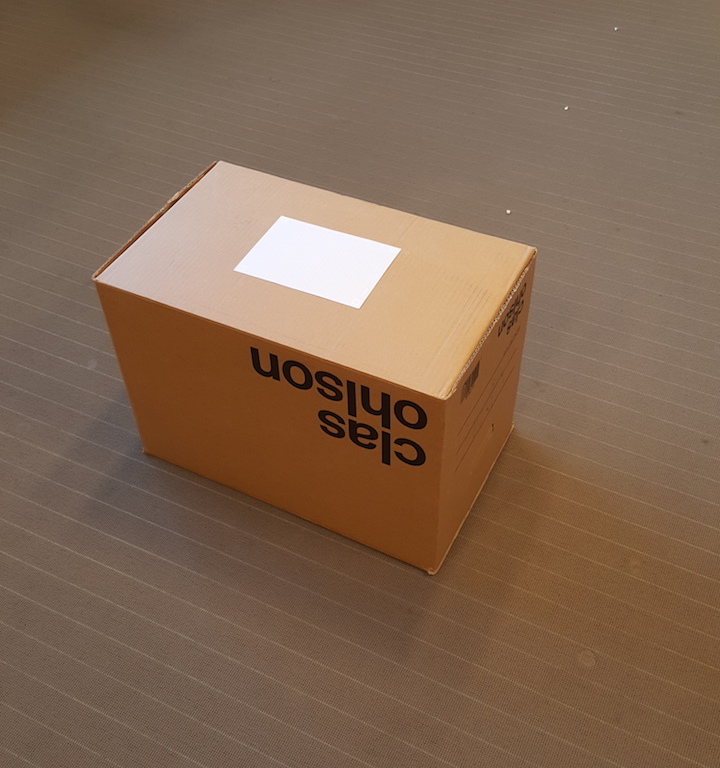
\includegraphics[width=\textwidth]{figures/angle_2.jpg}
		\label{fig:angle_2}
	\end{subfigure}
	~
	\begin{subfigure}[b]{0.2\textwidth}
		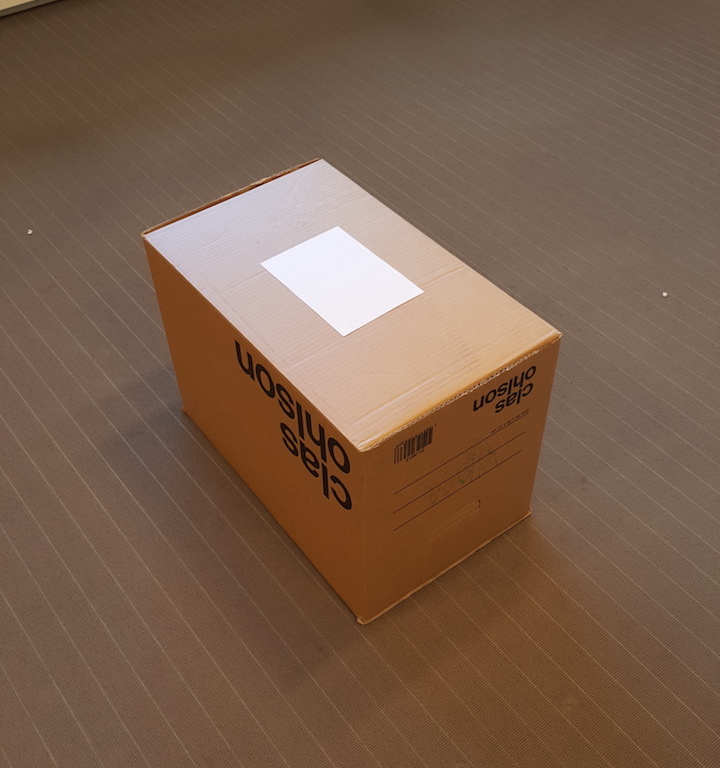
\includegraphics[width=\textwidth]{figures/angle_3.jpg}
		\label{fig:angle_3}
	\end{subfigure}
	
	\begin{subfigure}[b]{0.2\textwidth}
		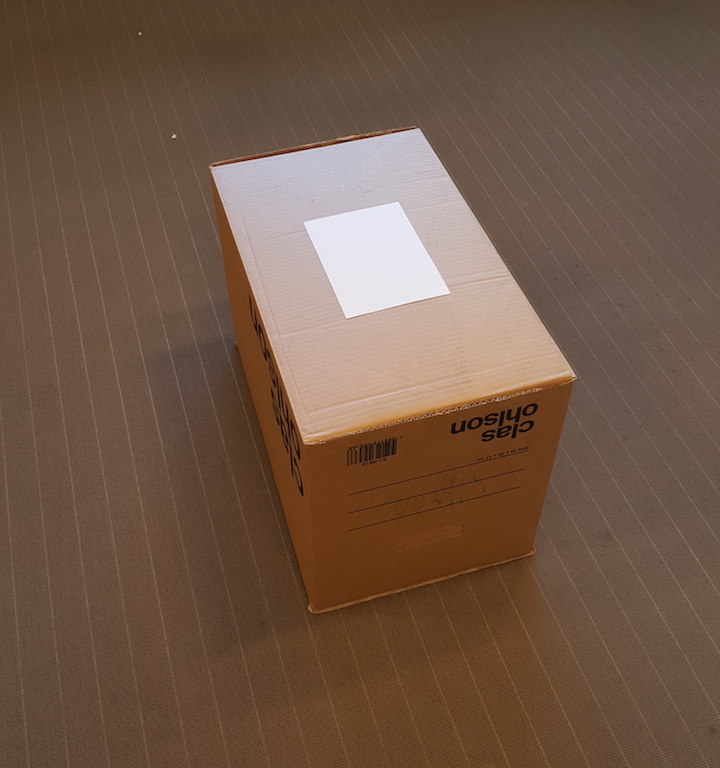
\includegraphics[width=\textwidth]{figures/angle_4.jpg}
		\label{fig:angle_4}
	\end{subfigure}
	~
	\begin{subfigure}[b]{0.2\textwidth}
		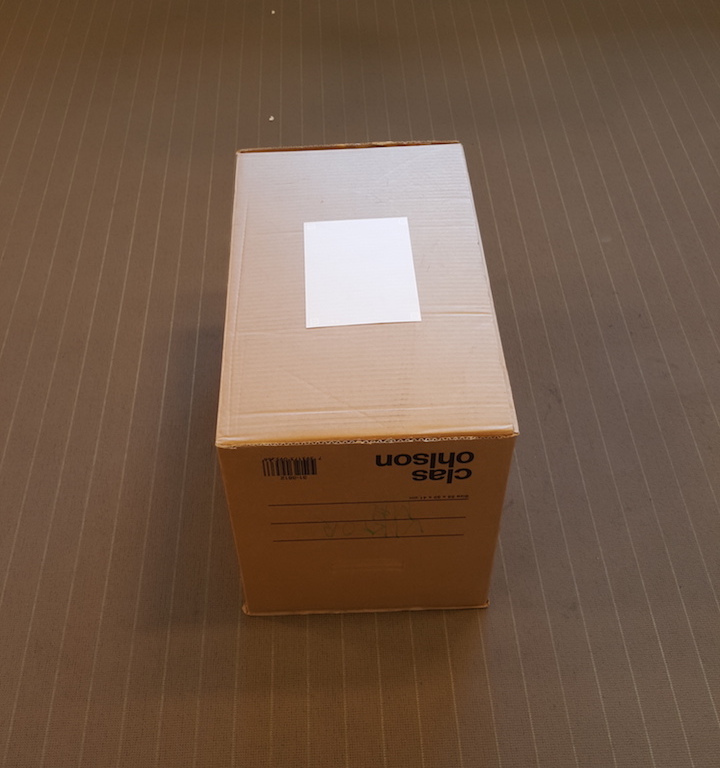
\includegraphics[width=\textwidth]{figures/angle_5.jpg}
		\label{fig:angle_5}
	\end{subfigure}
	\caption{Package 1 observed from the five different rotations.}\label{fig:positions}
\end{figure}